\chapter{Análisis del problema y requisitos}
\label{ch:analisis_problema}

% Este capítulo cubre el apartado "Análisis del problema" de la guía: identificación
% detallada del problema y requisitos que debe cumplir la solución.

\section{Descripción detallada del problema}
\label{sec:descripcion_problema}

El problema que aborda Harmony Hub no se limita a la recomendación musical en sentido clásico. La cuestión de fondo es otra: muchas personas utilizan la música como una herramienta espontánea para regular su estado interno, pero lo hacen dentro de entornos digitales que no siempre interpretan bien qué necesitan en ese momento.

En la práctica, esto genera una fricción recurrente. El usuario quiere concentrarse, bajar revoluciones, sentirse acompañado o recuperar energía, pero para llegar a una escucha que realmente encaje tiene que invertir tiempo en buscar, probar, descartar y reorganizar canciones o playlists. Ese esfuerzo previo contradice precisamente el efecto que se busca: claridad, alivio o foco.

Desde el punto de vista técnico, el problema puede descomponerse en varias necesidades encadenadas:

\begin{itemize}
    \item captar de forma breve el estado actual del usuario sin convertir la interacción en un cuestionario pesado;
    \item traducir ese estado a una recomendación musical con sentido funcional, no solo estético;
    \item materializar la recomendación en una playlist real y reproducible dentro de una plataforma de uso cotidiano;
    \item registrar el resultado de la experiencia para poder aprender de sesiones anteriores;
    \item hacerlo todo dentro de una experiencia móvil comprensible, rápida y suficientemente robusta.
\end{itemize}

Además, aparecen restricciones reales que condicionan el diseño. Por ejemplo, la recomendación no puede depender de largos y complejos cuestionarios, debido a que el uso de la app debe ser cotidiano y user-friendly. Tampoco conviene que la fase central de ranking musical quede totalmente subordinada a la plataforma externa, ya que la integración con Spotify está sujeta a permisos, disponibilidad de endpoints, limitaciones propias de su API y posibles restricciones de cuota o rate limit. Por eso la solución necesita un catálogo musical propio sobre el que apoyar la decisión principal y reservar Spotify para la autenticación y la materialización final. A eso se suma una cuestión importante: el sistema debe ser útil incluso cuando su capa de aprendizaje todavía no dispone de suficientes datos para activarse con garantías, tanto en términos globales como para el estado emocional concreto que se pretende recomendar.

Si se observa desde la perspectiva del usuario, el problema se puede resumir en una idea muy concreta: existe una distancia entre ``tener acceso a mucha música'' y ``recibir una propuesta musical adecuada para este momento''. Harmony Hub trata precisamente de reducir esa distancia.

\section{Actores y perfiles de usuario}
\label{sec:actores}

Aunque el usuario final es el actor central del sistema, la solución depende también de varios servicios y elementos externos que participan en el flujo completo. Tenerlos identificados ayuda a entender mejor dónde empieza y dónde termina la responsabilidad real de la aplicación.

\begin{table}[H]
\centering
\small
\renewcommand{\arraystretch}{1.1}
\begin{tabularx}{\textwidth}{|P{3.4cm}|Y|}
\hline
\textbf{Actor} & \textbf{Descripción} \\
\hline
Usuario final & Persona que utiliza Harmony Hub para realizar un check-in, recibir una recomendación de sesión, generar una playlist, consultar el historial y aportar feedback. Es el actor principal y el origen de casi todas las interacciones del sistema. \\
\hline
Backend de Harmony Hub & Servicio intermedio que procesa el contexto recibido desde la app, genera la recomendación, coordina el aprendizaje y conecta la lógica propia con servicios externos. \\
\hline
Spotify & Servicio externo utilizado para autenticación vinculada a música, consulta del perfil musical del usuario y materialización de playlists reales en su cuenta. \\
\hline
Firebase/Firestore & Servicio de persistencia empleado para almacenar información de sesiones, playlists generadas, datos históricos y documentos de apoyo al aprendizaje del sistema. \\
\hline
Modelo de aprendizaje de sesión & Componente lógico que, cuando existe suficiente evidencia, ayuda a ponderar mejor qué tipo de recomendación de sesión resulta más útil en contextos similares. No actúa siempre; está condicionado por criterios objetivos de activación sobre datos disponibles, calidad global y confianza operativa en la sesión. \\
\hline
\end{tabularx}
\caption{Actores identificados.}
\label{tab:actores}
\end{table}

Desde el punto de vista del perfil de uso, el actor principal puede describirse como una persona que ya convive con la escucha musical digital, que no busca necesariamente una herramienta clínica y que valora especialmente tres cosas: rapidez, sensación de acompañamiento y utilidad práctica. No necesita que el sistema le explique teoría sobre bienestar; necesita que le ayude a encontrar una sesión que encaje con su momento actual.

\section{Requisitos funcionales}
\label{sec:requisitos_funcionales}

Los requisitos funcionales describen qué debe ser capaz de hacer el sistema para responder al problema planteado.

\begin{table}[H]
\centering
\small
\renewcommand{\arraystretch}{1.1}
\begin{tabularx}{\textwidth}{|P{1.5cm}|Y|}
\hline
\textbf{ID} & \textbf{Requisito funcional} \\
\hline
RF1 & El sistema deberá permitir al usuario registrarse, iniciar sesión y cerrar sesión de forma segura. \\
\hline
RF2 & El sistema deberá permitir la recuperación de contraseña para restablecer el acceso a la cuenta. \\
\hline
RF3 & El sistema deberá recoger un check-in breve con información contextual relevante, al menos sobre estado de ánimo, objetivo de la sesión, nivel de energía y nivel de estrés. \\
\hline
RF4 & El sistema deberá permitir incluir variables adicionales de contexto, como preferencias vocales, intensidad deseada, exploración o popularidad. \\
\hline
RF5 & El sistema deberá generar una recomendación de sesión a partir del contexto declarado por el usuario. \\
\hline
RF6 & El sistema deberá vincular la recomendación generada con un identificador de sesión que permita trazar después la playlist y el feedback asociados. \\
\hline
RF7 & El sistema deberá permitir conectar la cuenta del usuario con Spotify. \\
\hline
RF8 & El sistema deberá generar una playlist real en Spotify a partir de la recomendación obtenida. \\
\hline
RF9 & El sistema deberá permitir consultar el historial de check-ins, playlists generadas y feedback asociado a sesiones anteriores. \\
\hline
RF10 & El sistema deberá permitir al usuario valorar si la sesión le ha resultado útil y registrar comentarios cualitativos sobre la experiencia. \\
\hline
RF11 & El sistema deberá almacenar la información necesaria para apoyar mecanismos de aprendizaje y personalización progresiva. \\
\hline
RF12 & El sistema deberá ofrecer modos rápidos o accesos predefinidos para situaciones recurrentes de uso. \\
\hline
\end{tabularx}
\caption{Requisitos funcionales de Harmony Hub.}
\label{tab:requisitos_funcionales}
\end{table}

\section{Requisitos no funcionales}
\label{sec:requisitos_no_funcionales}

Además de funcionar, Harmony Hub debe hacerlo con unas condiciones mínimas de calidad técnica y de experiencia.

\begin{table}[H]
\centering
\small
\renewcommand{\arraystretch}{1.1}
\begin{tabularx}{\textwidth}{|P{1.7cm}|Y|}
\hline
\textbf{ID} & \textbf{Requisito no funcional} \\
\hline
RNF1 & El sistema deberá ofrecer una experiencia de uso sencilla y comprensible en dispositivos móviles, evitando flujos innecesariamente largos. \\
\hline
RNF2 & El sistema deberá responder en tiempos razonables para no romper la sensación de continuidad entre check-in, recomendación y generación de playlist. \\
\hline
RNF3 & El sistema deberá mantener la trazabilidad entre recomendación, playlist y feedback, de forma que cada sesión pueda analizarse posteriormente. \\
\hline
RNF4 & El sistema deberá proteger el acceso del usuario mediante autenticación y no exponer datos sensibles de sesión de forma pública. \\
\hline
RNF5 & El sistema deberá depender de integraciones externas de manera controlada, gestionando errores de Spotify o de red, incluidos casos de rate limit o materialización fallida de pistas, sin bloquear por completo la experiencia ni comprometer la fase principal de ranking musical. \\
\hline
RNF6 & El sistema deberá ser mantenible, con una separación clara entre frontend, backend, persistencia y lógica de recomendación. \\
\hline
RNF7 & El sistema deberá permitir evolucionar el componente de aprendizaje sin rehacer la arquitectura principal de la solución. \\
\hline
RNF8 & El sistema deberá seguir siendo operativo aunque el modelo de aprendizaje no esté activado, utilizando reglas y lógica heurística como respaldo y permitiendo la abstención del componente aprendido cuando la evidencia no supere sus puertas de calidad. \\
\hline
RNF9 & El sistema deberá registrar evidencia suficiente para evaluar objetivamente el comportamiento del componente de aprendizaje cuando se disponga de datos adecuados, incluyendo señales que permitan decidir si la activación del aprendizaje es válida para cada mood. \\
\hline
\end{tabularx}
\caption{Requisitos no funcionales de Harmony Hub.}
\label{tab:requisitos_no_funcionales}
\end{table}

\section{Requisitos de información}
\label{sec:requisitos_informacion}

Además de definir qué debe hacer el sistema, conviene precisar qué información
necesita para poder hacerlo. En Harmony Hub esto es especialmente importante,
porque la personalización musical, la trazabilidad entre sesión y feedback y el
aprendizaje progresivo dependen de que determinadas piezas de información estén
presentes, bien delimitadas y almacenadas con el nivel de sensibilidad
adecuado.

\begin{table}[H]
\centering
\footnotesize
\renewcommand{\arraystretch}{1.1}
\setlength{\tabcolsep}{3.5pt}
\begin{tabularx}{\textwidth}{|P{1.1cm}|Y|}
\hline
\textbf{ID} & \textbf{Información requerida} \\
\hline
RI1 & Identidad básica de usuario (UID, correo, sesión autenticada). \\
\hline
RI2 & Estado de ánimo, objetivo, estrés y energía declarados en el check-in. \\
\hline
RI3 & Preferencias de sesión: voz, intensidad, exploración, popularidad, duración y resultado buscado. \\
\hline
RI4 & Contexto acústico resumido: categoría de ruido, medias y variabilidad. \\
\hline
RI5 & Datos de recomendación: modo propuesto, objetivos musicales y origen de selección. \\
\hline
RI6 & Datos de playlist generada: identificador, URL, número de pistas y resumen de selección. \\
\hline
RI7 & Feedback global de utilidad y estado posterior a la sesión. \\
\hline
RI8 & Perfil musical derivado y estadísticas agregadas. \\
\hline
RI9 & Ejemplos de entrenamiento a nivel de sesión. \\
\hline
\end{tabularx}
\caption{Requisitos de información principales de Harmony Hub.}
\label{tab:requisitos_informacion}
\end{table}

\section{Casos de uso}
\label{sec:casos_uso}

El análisis funcional de Harmony Hub se apoya en un diagrama general de casos
de uso y en una descripción textual de los flujos más relevantes. Esta
combinación permite resumir qué puede hacer el usuario dentro del sistema y, al
mismo tiempo, conservar una lectura bastante clara del recorrido principal de la
aplicación.

La \textbf{Figura~\ref{fig:casos_uso_general}} recoge una vista general de los
casos de uso principales de Harmony Hub. No intenta modelar cada pantalla de
forma aislada, sino representar las interacciones más relevantes del sistema:
acceso, check-in, recomendación, generación de playlist, consulta del historial
y cierre del ciclo mediante feedback.

\begin{figure}[H]
    \centering
    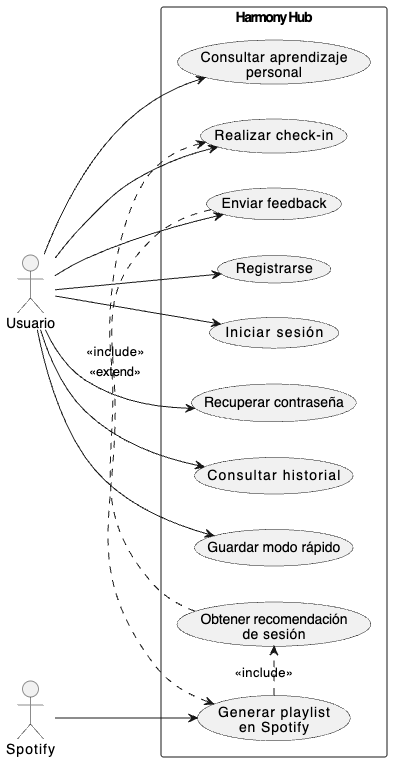
\includegraphics[width=0.52\linewidth]{Imagenes/diagrama_casos_uso.png}
    \caption{Diagrama general de casos de uso de Harmony Hub.}
    \label{fig:casos_uso_general}
\end{figure}

\subsection*{Casos de uso principales descritos}

Siguiendo el orden funcional del sistema, conviene resumir primero el acceso,
después la vinculación con Spotify, a continuación el flujo principal de sesión
y, por último, las funcionalidades de seguimiento, memoria y aprendizaje. Para
facilitar la lectura y la referencia cruzada posterior, cada caso de uso
principal se recoge en una tabla independiente y se acompaña de su diagrama
específico.

\begin{table}[H]
\centering
\small
\renewcommand{\arraystretch}{1.1}
\begin{tabularx}{\textwidth}{|P{1.1cm}|P{2.8cm}|P{1.4cm}|P{3.4cm}|Y|}
\hline
\textbf{ID} & \textbf{Caso de uso} & \textbf{Actor} & \textbf{Precondición} & \textbf{Resultado esperado} \\
\hline
CU1 & Registrarse e iniciar sesión & Usuario & El usuario dispone de la app y no mantiene sesión válida activa. & Se crea o valida la cuenta y se habilita el acceso a la pantalla principal. \\
\hline
\end{tabularx}
\caption{Caso de uso CU1: registrarse e iniciar sesión.}
\label{tab:caso_uso_cu1}
\end{table}

\begin{figure}[H]
    \centering
    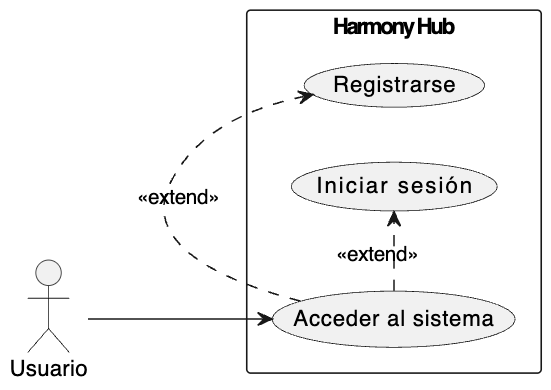
\includegraphics[width=0.54\linewidth]{Imagenes/caso_uso_cu1.png}
    \caption{Diagrama específico del caso de uso CU1: registrarse e iniciar sesión.}
    \label{fig:caso_uso_cu1}
\end{figure}

\begin{table}[H]
\centering
\small
\renewcommand{\arraystretch}{1.1}
\begin{tabularx}{\textwidth}{|P{1.1cm}|P{2.8cm}|P{1.4cm}|P{3.4cm}|Y|}
\hline
\textbf{ID} & \textbf{Caso de uso} & \textbf{Actor} & \textbf{Precondición} & \textbf{Resultado esperado} \\
\hline
CU2 & Recuperar contraseña & Usuario & El usuario ha olvidado la contraseña, pero recuerda el correo asociado. & El sistema envía el enlace de restablecimiento y la cuenta sigue siendo recuperable. \\
\hline
\end{tabularx}
\caption{Caso de uso CU2: recuperar contraseña.}
\label{tab:caso_uso_cu2}
\end{table}

\begin{figure}[H]
    \centering
    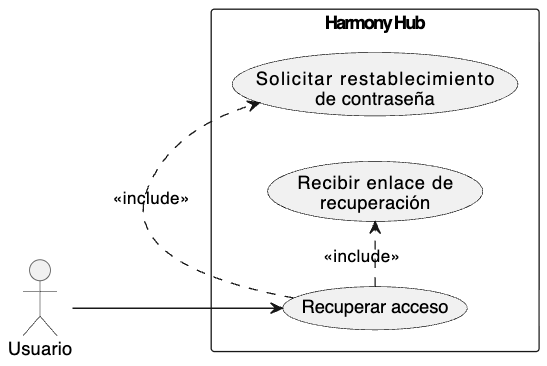
\includegraphics[width=0.54\linewidth]{Imagenes/caso_uso_cu2.png}
    \caption{Diagrama específico del caso de uso CU2: recuperar contraseña.}
    \label{fig:caso_uso_cu2}
\end{figure}

\begin{table}[H]
\centering
\small
\renewcommand{\arraystretch}{1.1}
\begin{tabularx}{\textwidth}{|P{1.1cm}|P{2.8cm}|P{1.4cm}|P{3.4cm}|Y|}
\hline
\textbf{ID} & \textbf{Caso de uso} & \textbf{Actor} & \textbf{Precondición} & \textbf{Resultado esperado} \\
\hline
CU3 & Conectar cuenta con Spotify & Usuario & El usuario ha iniciado sesión en Harmony Hub y todavía no ha vinculado su cuenta musical. & La cuenta de Spotify queda autorizada y disponible para generar playlists reales. \\
\hline
\end{tabularx}
\caption{Caso de uso CU3: conectar cuenta con Spotify.}
\label{tab:caso_uso_cu3}
\end{table}

\begin{figure}[H]
    \centering
    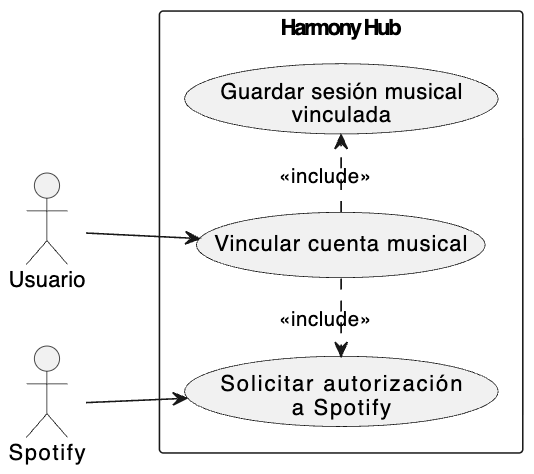
\includegraphics[width=0.54\linewidth]{Imagenes/caso_uso_cu3.png}
    \caption{Diagrama específico del caso de uso CU3: conectar cuenta con Spotify.}
    \label{fig:caso_uso_cu3}
\end{figure}

\begin{table}[H]
\centering
\small
\renewcommand{\arraystretch}{1.1}
\begin{tabularx}{\textwidth}{|P{1.1cm}|P{2.8cm}|P{1.4cm}|P{3.4cm}|Y|}
\hline
\textbf{ID} & \textbf{Caso de uso} & \textbf{Actor} & \textbf{Precondición} & \textbf{Resultado esperado} \\
\hline
CU4 & Realizar una sesión musical contextual & Usuario & El usuario ha iniciado sesión y tiene acceso operativo a la app. & Se registra el check-in, se genera la recomendación y se crea una playlist trazable. \\
\hline
\end{tabularx}
\caption{Caso de uso CU4: realizar una sesión musical contextual.}
\label{tab:caso_uso_cu4}
\end{table}

\begin{figure}[H]
    \centering
    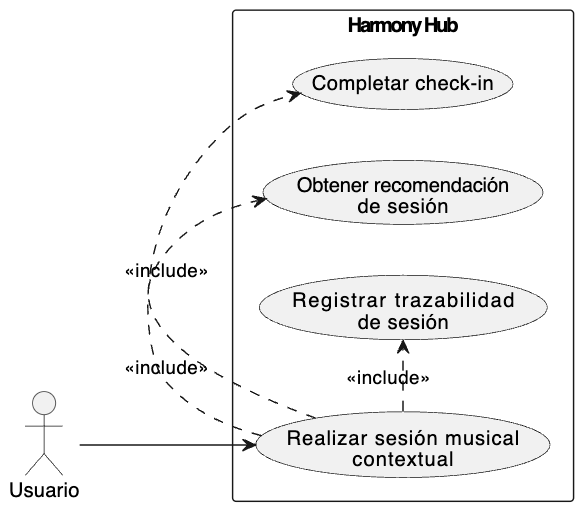
\includegraphics[width=0.54\linewidth]{Imagenes/caso_uso_cu4.png}
    \caption{Diagrama específico del caso de uso CU4: realizar una sesión musical contextual.}
    \label{fig:caso_uso_cu4}
\end{figure}

\begin{table}[H]
\centering
\small
\renewcommand{\arraystretch}{1.1}
\begin{tabularx}{\textwidth}{|P{1.1cm}|P{2.8cm}|P{1.4cm}|P{3.4cm}|Y|}
\hline
\textbf{ID} & \textbf{Caso de uso} & \textbf{Actor} & \textbf{Precondición} & \textbf{Resultado esperado} \\
\hline
CU5 & Consultar historial personal & Usuario & Existen sesiones registradas previamente. & El usuario puede revisar check-ins, playlists y feedback asociados. \\
\hline
\end{tabularx}
\caption{Caso de uso CU5: consultar historial personal.}
\label{tab:caso_uso_cu5}
\end{table}

\begin{figure}[H]
    \centering
    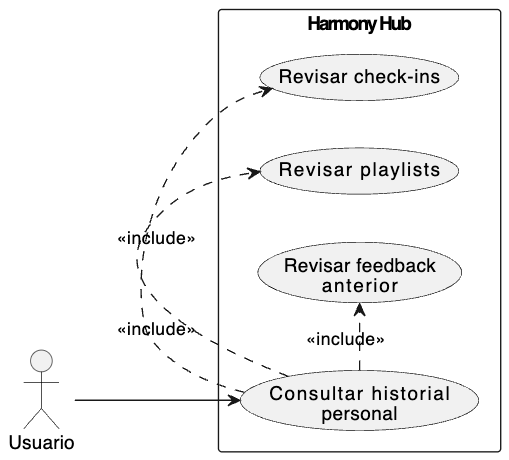
\includegraphics[width=0.54\linewidth]{Imagenes/caso_uso_cu5.png}
    \caption{Diagrama específico del caso de uso CU5: consultar historial personal.}
    \label{fig:caso_uso_cu5}
\end{figure}

\begin{table}[H]
\centering
\small
\renewcommand{\arraystretch}{1.1}
\begin{tabularx}{\textwidth}{|P{1.1cm}|P{2.8cm}|P{1.4cm}|P{3.4cm}|Y|}
\hline
\textbf{ID} & \textbf{Caso de uso} & \textbf{Actor} & \textbf{Precondición} & \textbf{Resultado esperado} \\
\hline
CU6 & Guardar un modo rápido & Usuario & El usuario navega por la sección de modos y detecta una situación reutilizable. & El modo queda almacenado como acceso rápido para uso posterior. \\
\hline
\end{tabularx}
\caption{Caso de uso CU6: guardar un modo rápido.}
\label{tab:caso_uso_cu6}
\end{table}

\begin{figure}[H]
    \centering
    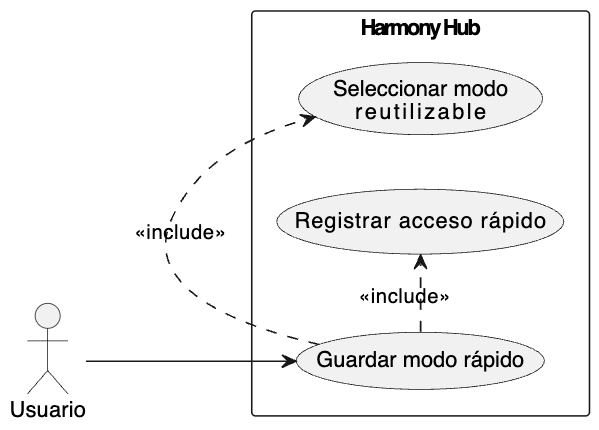
\includegraphics[width=0.54\linewidth]{Imagenes/caso_uso_cu6.png}
    \caption{Diagrama específico del caso de uso CU6: guardar un modo rápido.}
    \label{fig:caso_uso_cu6}
\end{figure}

\begin{table}[H]
\centering
\small
\renewcommand{\arraystretch}{1.1}
\begin{tabularx}{\textwidth}{|P{1.1cm}|P{2.8cm}|P{1.4cm}|P{3.4cm}|Y|}
\hline
\textbf{ID} & \textbf{Caso de uso} & \textbf{Actor} & \textbf{Precondición} & \textbf{Resultado esperado} \\
\hline
CU7 & Enviar feedback sobre una sesión & Usuario & Existe una recomendación o playlist generada asociada a la sesión. & La sesión queda cerrada con valoración y disponible para aprendizaje posterior. \\
\hline
\end{tabularx}
\caption{Caso de uso CU7: enviar feedback sobre una sesión.}
\label{tab:caso_uso_cu7}
\end{table}

\begin{figure}[H]
    \centering
    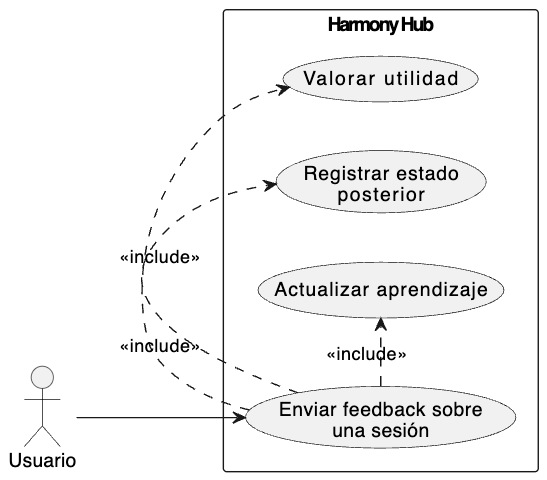
\includegraphics[width=0.54\linewidth]{Imagenes/caso_uso_cu7.png}
    \caption{Diagrama específico del caso de uso CU7: enviar feedback sobre una sesión.}
    \label{fig:caso_uso_cu7}
\end{figure}

\begin{table}[H]
\centering
\small
\renewcommand{\arraystretch}{1.1}
\begin{tabularx}{\textwidth}{|P{1.1cm}|P{2.8cm}|P{1.4cm}|P{3.4cm}|Y|}
\hline
\textbf{ID} & \textbf{Caso de uso} & \textbf{Actor} & \textbf{Precondición} & \textbf{Resultado esperado} \\
\hline
CU8 & Consultar aprendizaje personal & Usuario & Existe actividad previa suficiente dentro del sistema. & El usuario accede a patrones e insights agregados sobre su historial de uso. \\
\hline
\end{tabularx}
\caption{Caso de uso CU8: consultar aprendizaje personal.}
\label{tab:caso_uso_cu8}
\end{table}

\begin{figure}[H]
    \centering
    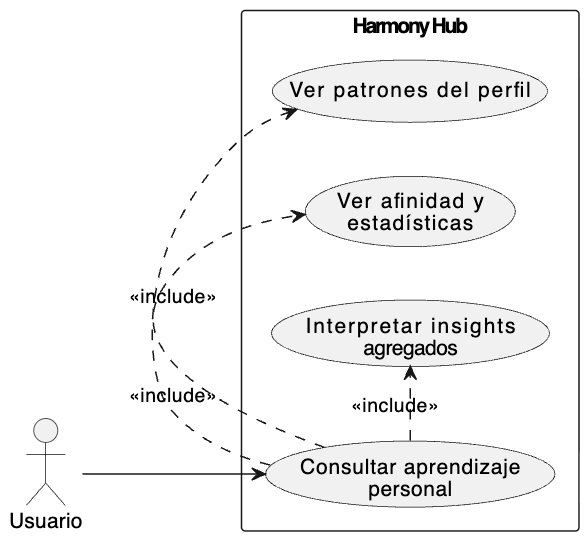
\includegraphics[width=0.54\linewidth]{Imagenes/caso_uso_cu8.png}
    \caption{Diagrama específico del caso de uso CU8: consultar aprendizaje personal.}
    \label{fig:caso_uso_cu8}
\end{figure}

\section{Matriz de trazabilidad}
\label{sec:matriz_trazabilidad}

Para reforzar la coherencia entre el análisis funcional y el comportamiento
esperado del sistema, la Tabla~\ref{tab:matriz_trazabilidad} reorganiza la
trazabilidad desde el punto de vista de los casos de uso principales. Para
facilitar la lectura, la matriz reduce la información a la relación directa
entre caso de uso y requisito, marcando con una X las coincidencias
correspondientes.

\begin{table}[H]
\centering
\scriptsize
\renewcommand{\arraystretch}{1.1}
\setlength{\tabcolsep}{2.8pt}
\resizebox{\textwidth}{!}{%
\begin{tabular}{|c|*{12}{c|}*{9}{c|}}
\hline
\textbf{CU} & \textbf{RF1} & \textbf{RF2} & \textbf{RF3} & \textbf{RF4} & \textbf{RF5} & \textbf{RF6} & \textbf{RF7} & \textbf{RF8} & \textbf{RF9} & \textbf{RF10} & \textbf{RF11} & \textbf{RF12} & \textbf{RNF1} & \textbf{RNF2} & \textbf{RNF3} & \textbf{RNF4} & \textbf{RNF5} & \textbf{RNF6} & \textbf{RNF7} & \textbf{RNF8} & \textbf{RNF9} \\
\hline
CU1 & X &  &  &  &  &  &  &  &  &  &  &  & X &  &  & X &  & X &  &  &  \\
\hline
CU2 &  & X &  &  &  &  &  &  &  &  &  &  & X &  &  & X &  &  &  &  &  \\
\hline
CU3 &  &  &  &  &  &  & X &  &  &  &  &  & X &  &  &  & X & X &  &  &  \\
\hline
CU4 &  &  & X & X & X & X &  & X &  &  &  &  & X & X & X &  & X &  &  & X & X \\
\hline
CU5 &  &  &  &  &  & X &  &  & X & X &  &  & X &  & X & X &  &  &  &  &  \\
\hline
CU6 &  &  &  &  &  &  &  &  &  &  &  & X & X &  &  &  &  & X &  &  &  \\
\hline
CU7 &  &  &  &  &  & X &  &  &  & X & X &  & X &  & X & X &  &  &  &  & X \\
\hline
CU8 &  &  &  &  &  &  &  &  & X &  & X &  & X &  &  &  &  &  &  & X & X \\
\hline
\end{tabular}}
\caption{Matriz de trazabilidad centrada en casos de uso y requisitos.}
\label{tab:matriz_trazabilidad}
\end{table}

\section{Restricciones y riesgos iniciales}
\label{sec:restricciones_riesgos}

El diseño de Harmony Hub está condicionado por varias restricciones que conviene reconocer desde el principio, ya que afectan tanto a la implementación como a la evaluación del sistema.

\textbf{Restricciones técnicas}
\begin{itemize}
    \item La integración con Spotify depende de permisos, disponibilidad y cambios en su API.
    \item Algunas capacidades avanzadas del ecosistema Spotify no siempre están disponibles en modo de desarrollo o pueden sufrir restricciones externas.
    \item La experiencia debe funcionar en móvil sin requerir sensores complejos ni hardware específico.
    \item El sistema de aprendizaje no puede asumirse como plenamente operativo desde el inicio, porque depende de disponer de suficiente volumen y equilibrio de datos etiquetados.
    \item La persistencia documental depende de reglas activas de Firestore y de la coherencia entre dichas reglas, los documentos generados por el cliente y los agregados escritos por backend.
    \item El análisis acústico del entorno debe limitarse a métricas resumidas y no a audio persistido, lo que restringe deliberadamente la profundidad del tratamiento posible sobre la señal.
\end{itemize}

\textbf{Restricciones de alcance}
\begin{itemize}
    \item El proyecto debe mantenerse dentro del marco temporal y técnico de un TFG.
    \item No se persigue construir un producto clínico, ni validar resultados terapéuticos, ni desarrollar un sistema musical universal.
    \item El aprendizaje se plantea a nivel de sesión, no como un modelo total de predicción del comportamiento musical del usuario.
    \item La evaluación longitudinal se concentra en un perfil principal de uso, lo que favorece la trazabilidad del aprendizaje pero limita la comparación entre perfiles heterogéneos.
\end{itemize}

\textbf{Riesgos iniciales}
\begin{itemize}
    \item \textbf{R1. Dependencia de servicios externos}. Si Spotify cambia un endpoint o restringe funcionalidades, parte del flujo puede verse afectado.
    \item \textbf{Mitigación}. Diseñar la arquitectura para que el backend mantenga el ranking principal sobre un catálogo propio y deje a Spotify sobre todo la fase de materialización final.
    \item \textbf{R2. Insuficiencia de datos para activar el modelo}. Un volumen bajo o desequilibrado de feedback puede impedir que el aprendizaje entre en producción con garantías.
    \item \textbf{Mitigación}. Mantener una puerta de activación objetiva y asegurar un modo heurístico funcional mientras se recopilan datos.
    \item \textbf{R3. Fricción de uso}. Si el check-in es demasiado largo o el flujo resulta poco claro, el usuario puede abandonar antes de cerrar la sesión con feedback.
    \item \textbf{Mitigación}. Priorizar una experiencia móvil breve, guiada y con jerarquía visual clara.
    \item \textbf{R4. Expectativas infladas sobre la personalización}. El usuario podría esperar una precisión muy alta desde las primeras sesiones.
    \item \textbf{Mitigación}. Diseñar el sistema como aprendizaje progresivo y dejar claro que mejora con el uso.
    \item \textbf{R5. Desalineación entre reglas documentales y cliente}. Un cambio menor en nombres de campos o colecciones puede bloquear escrituras críticas como feedback o persistencia privada.
    \item \textbf{Mitigación}. Mantener validaciones explícitas, revisar \texttt{firestore.rules} junto con los servicios Flutter y comprobar el flujo completo con pruebas manuales de extremo a extremo.
    \item \textbf{R6. Cobertura insuficiente del catálogo local}. Un catálogo estructurado todavía limitado puede dejar algunos contextos con menor variedad o con materialización más difícil en Spotify.
    \item \textbf{Mitigación}. Enriquecer progresivamente \texttt{msd\_tracks}, documentar mecanismos de \textit{fallback} y mantener la separación entre ranking local y materialización externa.
\end{itemize}

En conjunto, estas restricciones no invalidan la solución. Ayudan a situarla con mayor precisión y a distinguir entre lo que el sistema ya resuelve, lo que resuelve parcialmente y lo que queda como evolución futura.
